\documentclass[12pt]{article}
\usepackage{amsmath,mathtools}
\usepackage[usenames,dvipsnames]{xcolor}
%\usepackage[bitstream-charter]{mathdesign}
%\usepackage{mathptmx}

\usepackage{textcomp}
\usepackage{cmbright}
\usepackage[german]{babel}
\usepackage{microtype}
%\usepackage{microtype}
\usepackage[utf8]{inputenc}
\usepackage[T1]{fontenc}
\usepackage{helvet}
\renewcommand{\familydefault}{\sfdefault}

\usepackage{siunitx}
%\usepackage{tikz}
\usepackage{fancyhdr}
\usepackage{sectsty}
\usepackage{setspace}
\usepackage{booktabs} % To thicken table lines
\usepackage[version=4]{mhchem}
\usepackage{textcomp}
\usepackage{tabulary}

\usepackage[ddmmyyyy]{datetime}
\renewcommand{\dateseparator}{.}

\pagestyle{fancy}

\cfoot{\thepage}

\lhead{Nevroz Arslan }
\rhead{03.02.2016}
\setlength{\headheight}{15pt}

\usepackage{overcite}
\renewcommand\citeform[1]{[#1]}

%\renewcommand*\printatom[1]{{\fontsize{10}{12}\selectfont\ensuremath{\mathsf{#1}}}}
\sectionfont{\fontsize{12}{15}\selectfont}

\makeatletter
    \setlength\@fptop{0\p@}
\makeatother


\newcommand\textbox[1]{%
  \parbox{.333\textwidth}{#1}%
}


\setlength{\headheight}{15pt}
\sisetup{detect-weight=true, detect-all}
\sisetup{text-celsius = $^\circ\mkern-1mu$C}


\renewcommand{\thesection}{\arabic{section}.}
\renewcommand{\thesubsection}{\thesection\arabic{subsection}}
\renewcommand{\headrulewidth}{0pt}


\begin{document}
%%%%%%%%%%%%%
\begin{onehalfspace}

\begingroup
\leftskip=0cm plus 0.5fil \rightskip=0cm plus -0.5fil
\parfillskip=0cm plus 1fil
 \textbf{\large Darstellung von \textit{N\textquotesingle,N\textquotesingle\textquotesingle}-Dicyclohexyl-\textit{N,N}-diethylguanidin}\par
\endgroup
\begin{center}
 \textbf{Präparat Nr. 5 von 7}
\end{center}
\section{Reaktionstyp: \textnormal{Addition} }
\begin{figure}[ht]
\centering
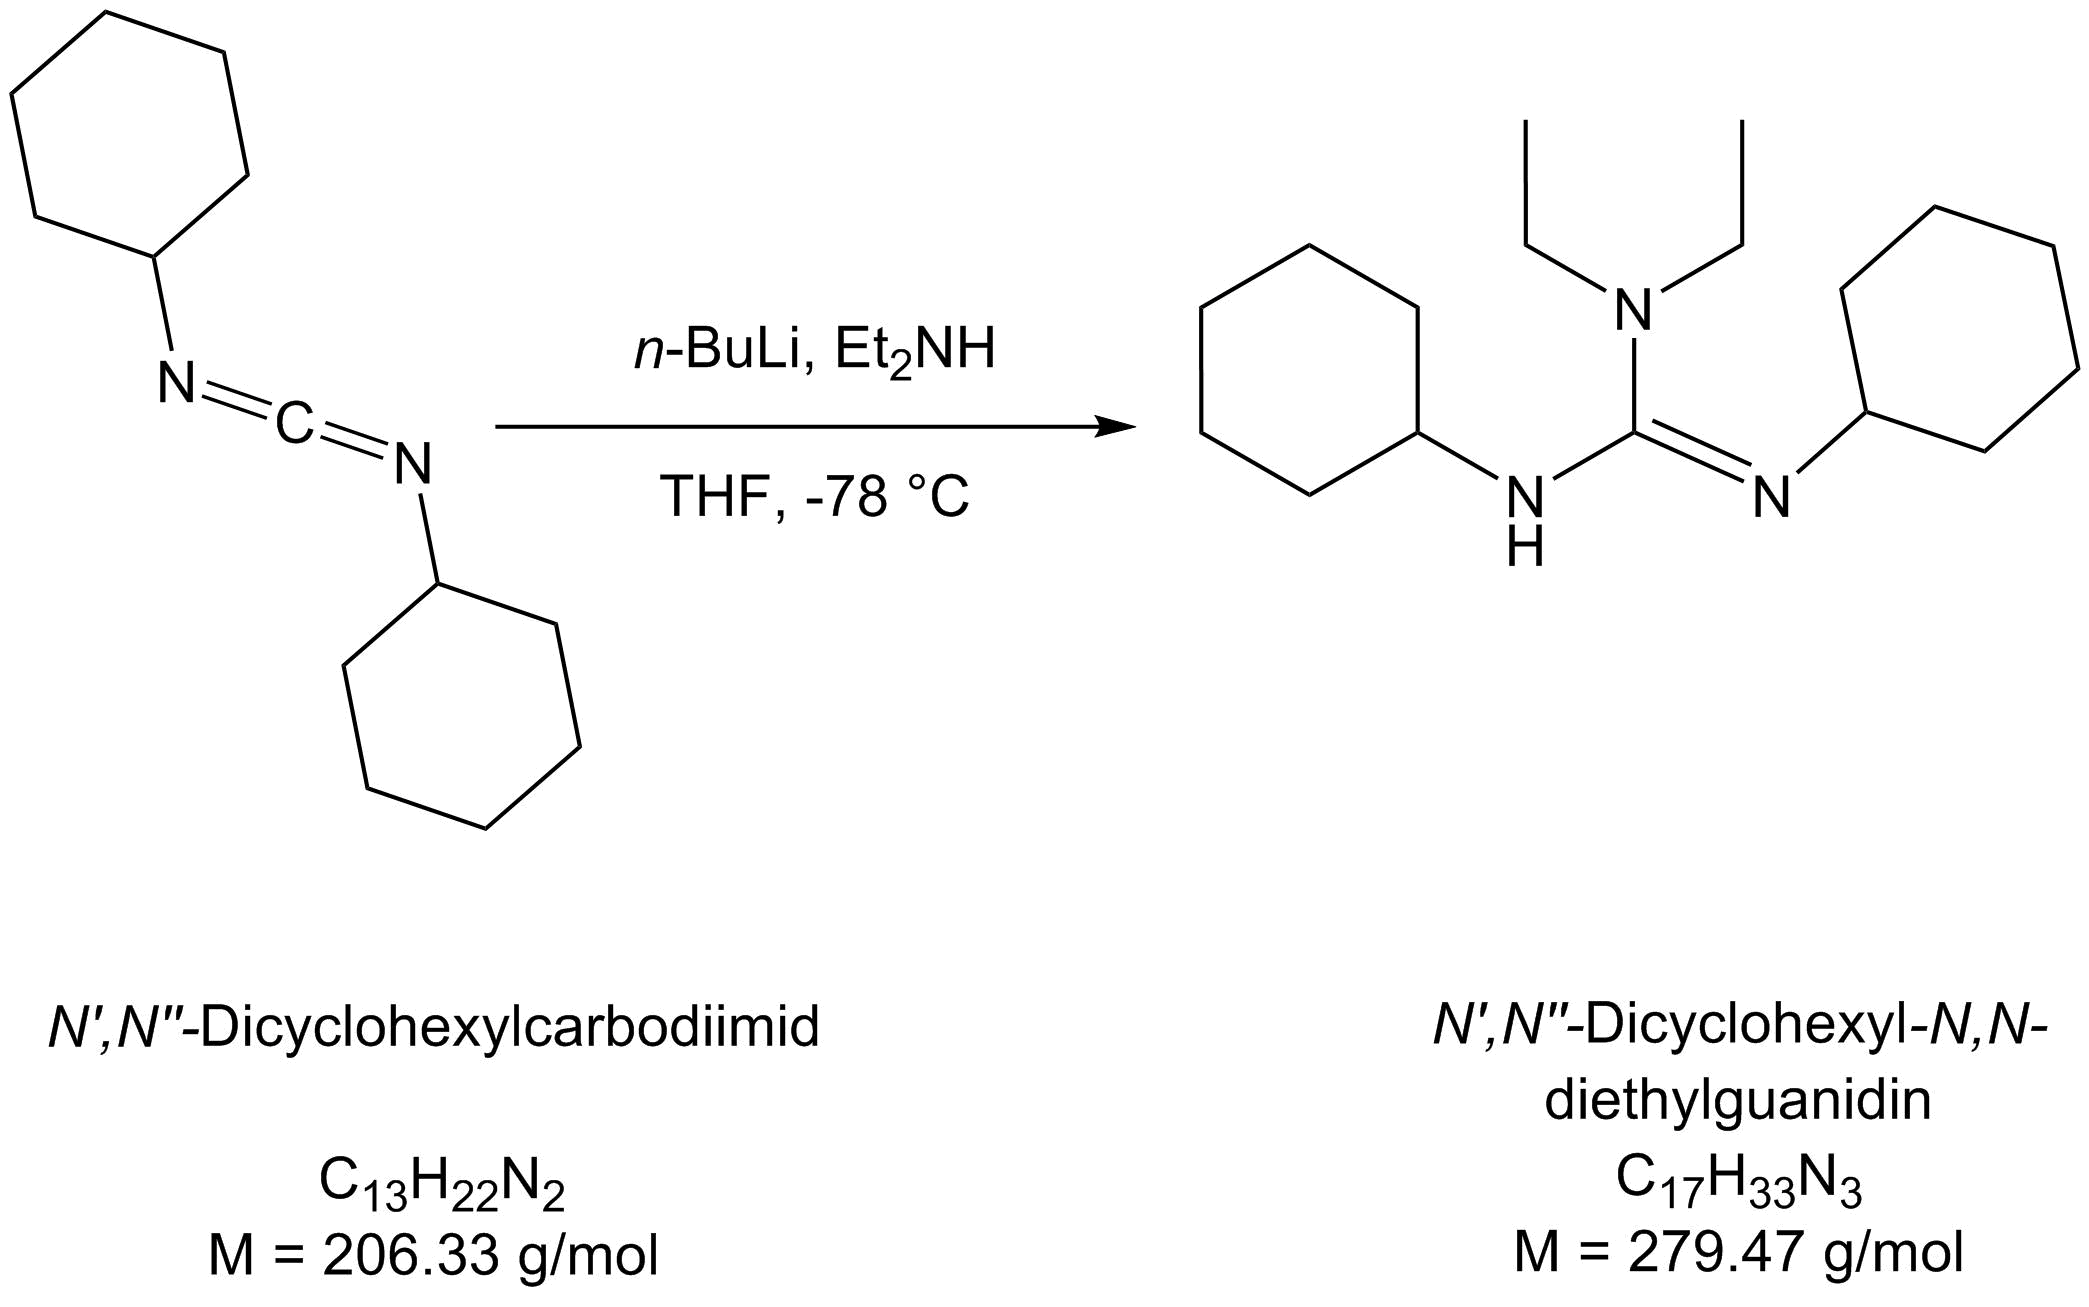
\includegraphics[width=\textwidth]{reaktion.png}
\end{figure}

%\chemabove{\lewis{2:,Si}}{\hspace{5mm}\scriptstyle\ominus}
%%%%%%%%%%%%%
% Berechnung des Ansatzes

\section{Berechnung des Ansatzes: }
Es sollte \textit{N\textquotesingle,N\textquotesingle\textquotesingle}-Dicyclohexyl-\textit{N,N}-diethylguanidin aus \textit{N,N}-Dicyclohexylcarb-odiimid (4.1 \si{\milli\liter}, 20 mmol) hergestellt werden. Die Umrechnung des Literaturansatzes ergab folgenden Ansatz:\cite{vor}\par
\noindent
\begin{tabulary}{26cm}{Lrrrr}
\toprule
\textbf{ Bezeichnung }&\textbf{M [\si{\gram\per\mol}]} & \textbf{ n [\si{\milli\mol}]} & \textbf{Menge} &  \textbf{Equiv}\\
\midrule
 \textit{N,N}-Dicyclohexylcarbodiimid & 206.33 & 20.0  & 4.13 \si{\gram} & 1.00 \\
 Diethylamin   & 73.14   &  40.0  &  4.2 \si{\milli\liter} & 2.00 \\
\textit{n}-Butyllithium    & 64.06   &  20.0  &  8.0 \si{\milli\liter} & 1.00 \\
 Tetrahydrofuran &   &  & 55  \si{\milli\liter}& LM \\
\bottomrule
\end{tabulary}

%%%%%%%%%%%%%
% Durchführung
%%%%%%%%%%%%%
\section{Durchführung \cite{vor}}
In einem ausgehizten 250 mL-Schlenkkolben wurde zunächst unter Schutzgas eine Lösung von Diethylamin (40.0 \si{\milli\mol}, 4.2 \si{\milli\liter}) in Tetrahydrofuran (30 \si{\milli\liter}) vorgelegt, mit einer Trockeneis-Aceton-Kältemischung auf -78 \si{\celsius} gekühlt und danach mit \textit{n}-Butyllithium (20.0 \si{\milli\mol}, 2.5 N, 8.0 \si{\milli\liter}) versetzt. Das Reaktionsgemisch wurde eine Stunde lang gerührt und dann wurde eine Lösung von \textit{N,N}-Dicyclohexylcarbodiimid (4.13 \si{\gram}, 20.0 \si{\milli\mol}) in Tetrahydrofuran (10 \si{\milli\liter}) hinzugetropft. Die Mischung wurde über Nacht bei Raumtemperatur unter Rühren stehen gelassen. Nach dem Hydrolysieren des Reaktionsgemisches mit kaltem Wasser (20 \si{\milli\liter}), wurde die organische Phase abgetrennt, über Magnesiumsulfat getrocknet und am Rotationsverdampfer eingeengt. Der Rückstand wurde in Hexan aufgenommen und anschließend filtriert. Die Lösung wurde erneut eingeengt. Das Rohprodukt wurde per Kugelrohr-Destillation (190 \si{\celsius}, 0.09 \si{\milli\bar}) aufgereinigt. Das Produkt (3.46 g, 12.4 mmol, 62 \%) wurde als farblose Flüssigkeit erhalten.
%%%%%%%%%%%%
% Ausbeute
%%%%%%%%%%%%%
\section{Ausbeute}
\begin{tabular}{ ll}
  5.58 \si{\gram} (20.0 \si{\milli\mol})   & = 100 \%\\
  3.46 \si{\gram} (12.4 \si{\milli\mol})   & = 62 \% (Lit.\cite{vor} : 67 \%) \\
 \end{tabular}
%%%%%%%%%%%%%
%Physikalische Daten des Produktes
%%%%%%%%%%%%%
%\section{Physikalische Daten des Produktes}
%\textit{2,2-Dimethyl-pent-4-enenitril}
\newpage

\section{Spektrenauswertung}
\begin{figure}[!htbp]
   \centering
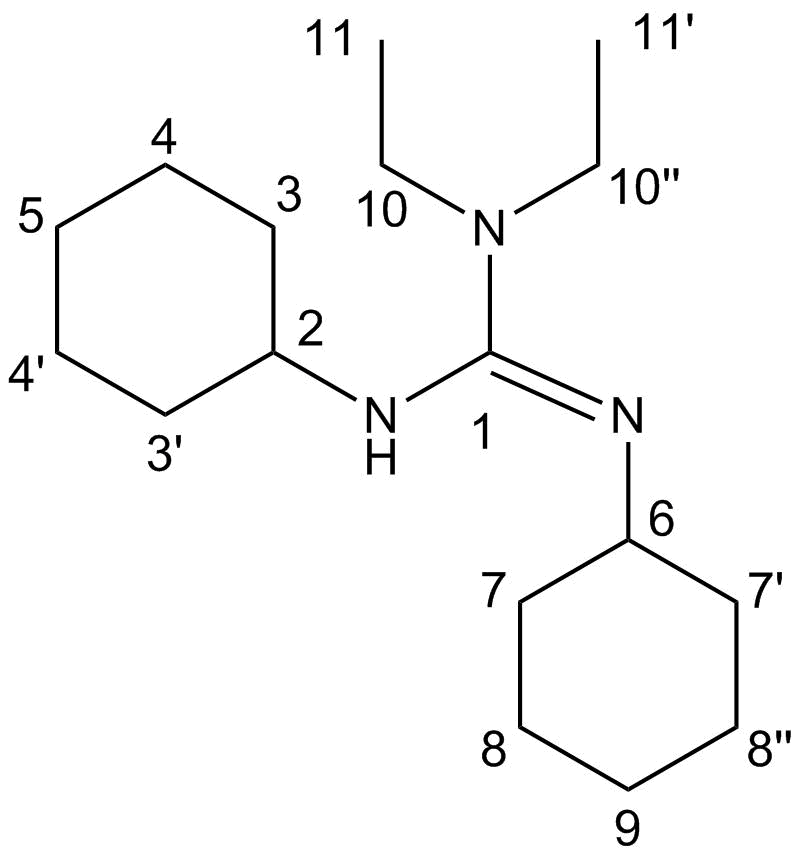
\includegraphics[scale=0.3]{auswert.png}
\end{figure}

\noindent
\textbf{\ce{^1_{}H-NMR}} (500 MHz, \ce{CDCl_3}): \sffamily \ce{$\delta$} =
0.96 (t, \ce{^3_{}\textit{J}} = 7.1 \si{\hertz}, 6 H, 11-H),
1.05 – 1.90 (m, 20 H, 3-H, 4-H, 5-H, 7-H, 8-H, 9-H), 
2.80 - 2.98 (m, 2 H, 2-H, 6-H),
3.03 (q, \ce{^3_{}\textit{J}} = 7.1 \si{\hertz}, 4 H, 10-H) ppm. \\
\noindent
\textbf{\ce{^{13}_{}C-NMR}} (125 MHz, DEPT, \ce{CDCl_3}): \sffamily \ce{$\delta$} =
12.7 (\ce{CH_3}, C-11),
24.6 + 25.4 + 25.7 (\ce{CH_2}, C-4, C-5, C-8, C-9),
34.8 (\ce{CH_2}, C-3, C-7),
42.6 (\ce{CH_2}, C-10),
77.3 (\ce{CH}, C-2, C-6),
153.9 (\ce{C}, C-1) ppm.
\section{Mechanismus\cite{bio}}

Im ersten Teil der Reaktion erfolgt die Deprotonierung eines sekundären Amins. 
 \textit{n}-Butyllithium (\textbf{1}) und Diethylamin (\textbf{2}) reagieren in einer
Säure-Base Reaktion zum Lithiumdiethylamid (\textbf{3}). Im zweiten Teil der Reaktion erfolgt eine nukleophile Additon.
Das Diethylamidanion aus (\textbf{3}) addiert an den elektropositiven Carbodiimid-Kohlenstoff des \textit{N,N}-Dicyclohexylcarbodiimids (\textbf{4}). Dabei entsteht ein Guanidinium-Ion \textbf{5}, welches durch die Mesomerie stark stabilisiert wird. Die Hydrolyse des Carbanions \textbf{5} liefert das gewünschte Produkt \textit{N\textquotesingle,N\textquotesingle\textquotesingle}-Dicyclohexyl-\textit{N,N}-diethylguanidin (\textbf{6}).
\begin{figure}[!htbp]
\centering
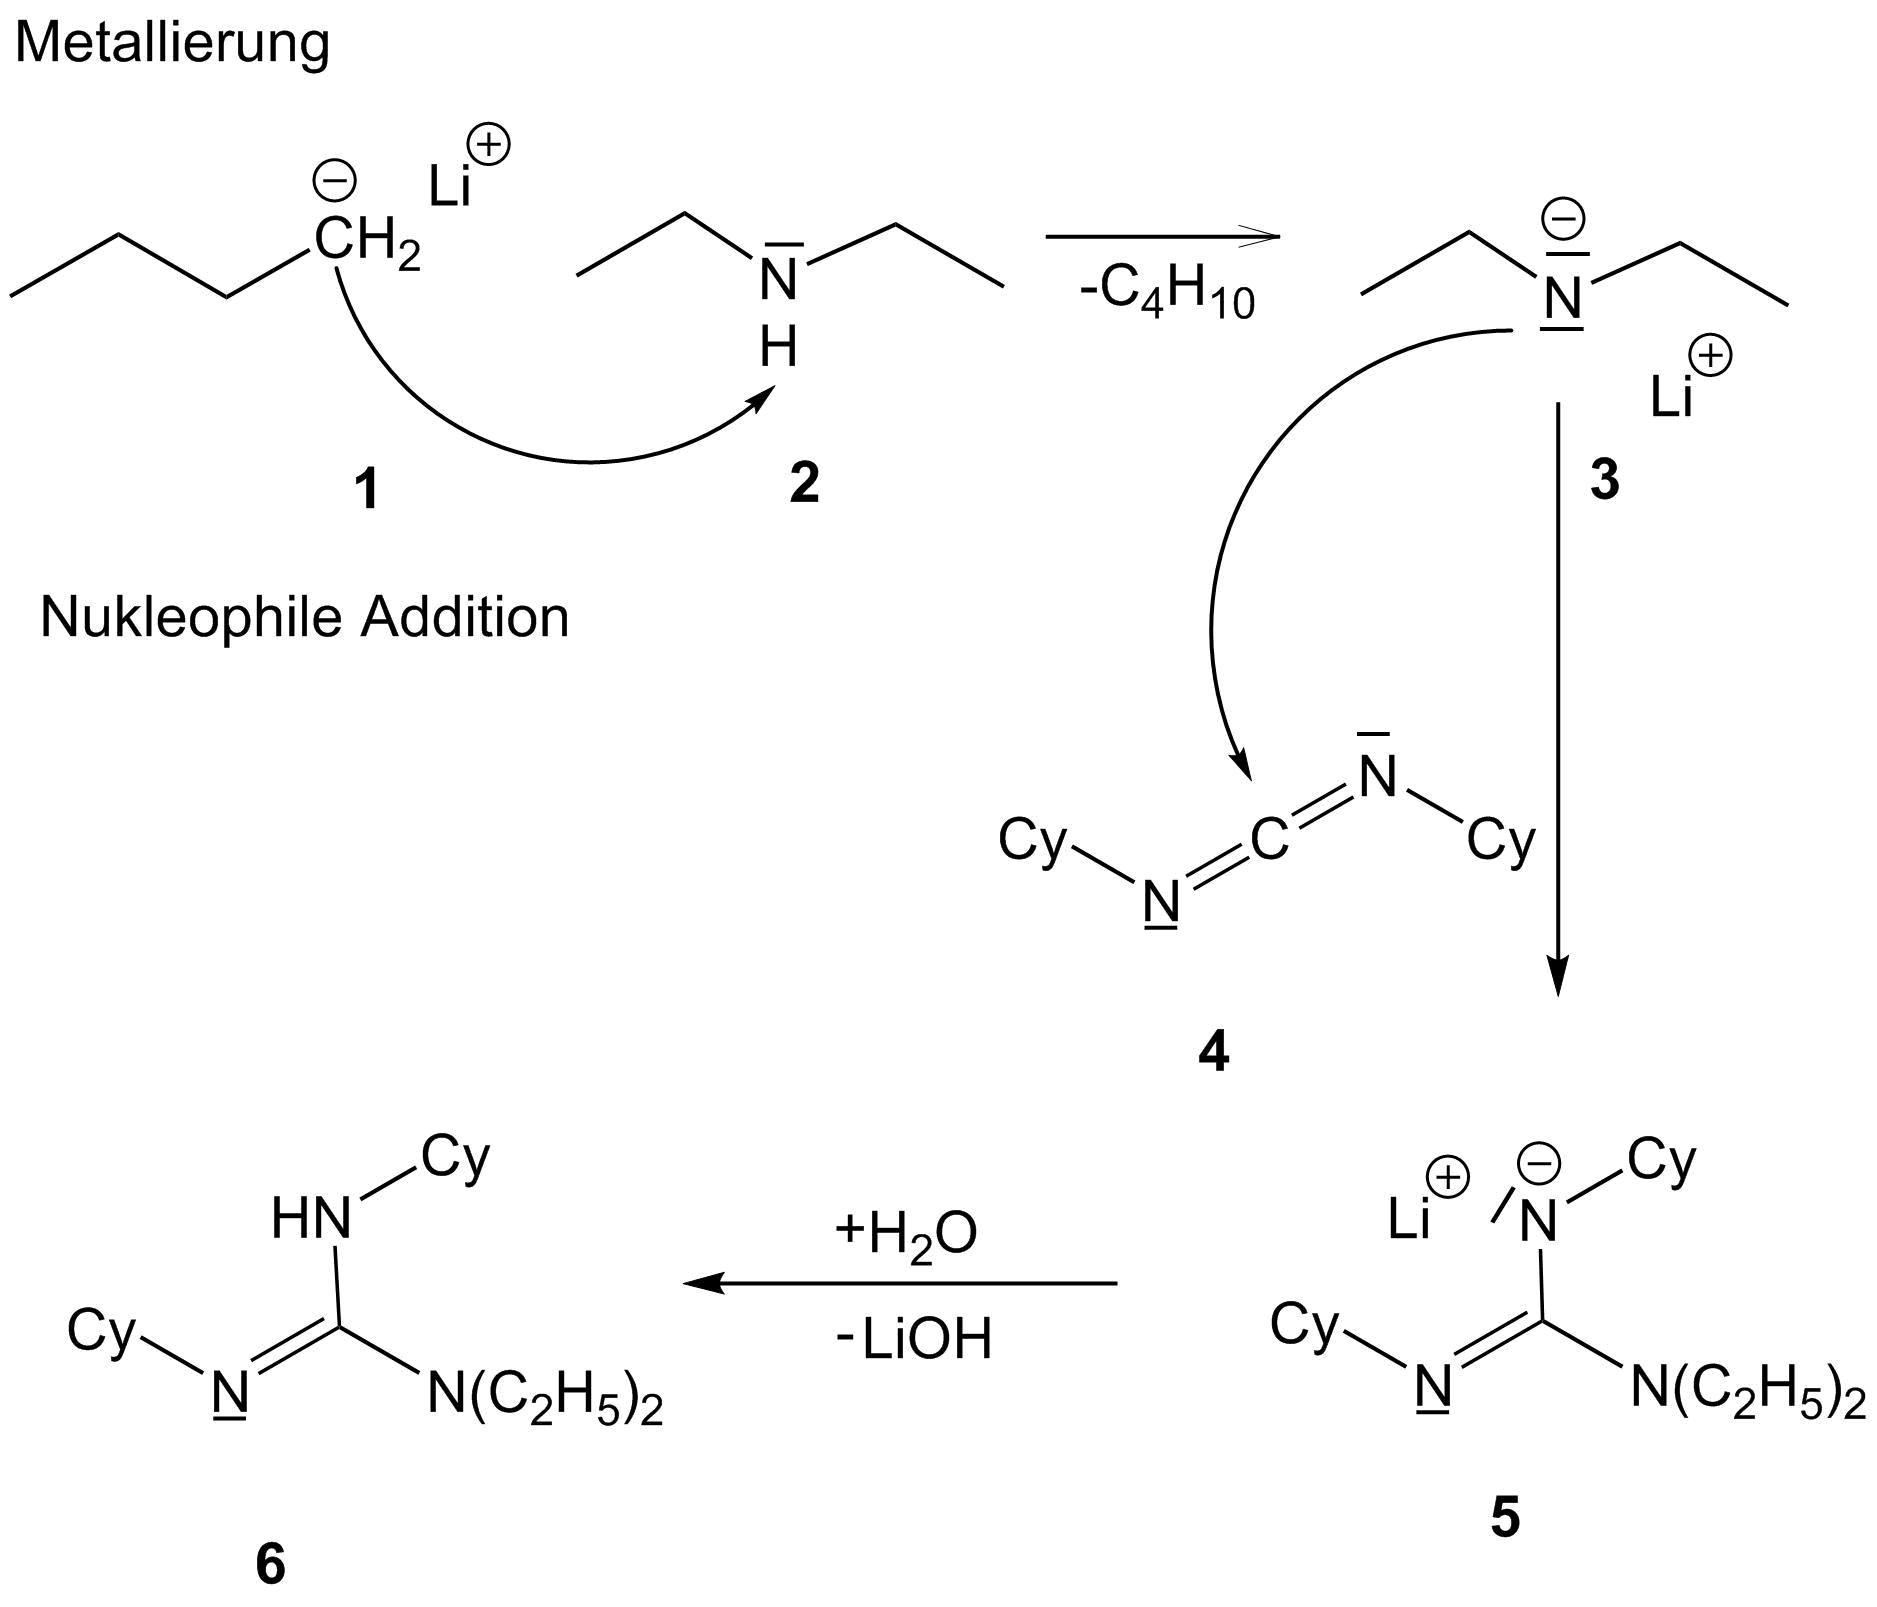
\includegraphics[width=0.9\textwidth]{mechan.png}
\end{figure}

\section{Abfallentsorgung}
Die nach dem Hydrolysieren verbleibenden wässrigen Phasen wurden
nach einer pH-Wertbestimmung im Behälter für basische wässrige Abfälle entsorgt.
Das im Rotationsverdampfer abgetrennte Lösungsmittel wurde im Behälter für halogenfreie Kohlenwasserstoffe entsorgt.
\section{Literatur}

\renewcommand{\section}[2]{}%
\def\bibindent{0em}
\begin{thebibliography}{99\kern\bibindent}
\makeatletter
\let\old@biblabel\@biblabel
\def\@biblabel#1{\old@biblabel{#1}\kern\bibindent}
\let\old@bibitem\bibitem
\def\bibitem#1{\old@bibitem{#1}\leavevmode\kern-\bibindent}
\makeatother
\bibitem{vor}
E. W. Thomas, E. E. Nishizawa, D. C. Zimmermann, D. J. Williams, \textit{
J. Med. Chem.} \textbf{1989}, \textit{32}, 228–236.
\bibitem{bio}
J. Buddrus, \textit{Grundlagen der Organische Chemie}, 4. Aufl., De Gruyter, Berlin \textbf{2011}, S. 481.
\end{thebibliography}
\end{onehalfspace}
\end{document}


